\documentclass{a0poster}
\usepackage[margin=0cm, paperwidth=90cm, paperheight=120cm]{geometry}
\usepackage{poster}
\usepackage{physics}
\usepackage[authoryear]{natbib}

\begin{document}
\begin{center}
    \colorbox{nottblue!0}{%
        \begin{minipage}[t]{\textwidth} 
            \vspace{0.8em}
            \begin{center}
                {\fontsize{80pt}{85pt}\selectfont\textbf{\textcolor{black}{Hofstadter butterfly in monolayer transistion metal dichalcogenides}}}\\[1ex] % Increased font size
               \Large \textit{\textcolor{black}{Huynh Thanh Duc}}\textsuperscript{\textcolor{black}{1}}, \textit{\textcolor{black}{Tran Khoi Nguyen}}\textsuperscript{\textcolor{black}{2}}, \textit{\textcolor{black}{Dao Duy Tung}}\textsuperscript{\textcolor{black}{2}}\\
    \textit{\textsuperscript{\textcolor{black}{1}}\textcolor{black}{Ho Chi Minh City Institute of Physics, Vietnam Academy of Science and Technology, 1 Mac Dinh Chi Street, District 1, Ho Chi Minh City, Vietnam }}\\
    \textit{\textsuperscript{\textcolor{black}{2}}\textcolor{black}{Department of Physics, University of Science, Vietnam National University Ho Chi Minh City,
     227 Nguyen Van Cu Street, District 5, Ho Chi Minh City, Vietnam }}\\
    \vspace{0em}
                \end{center}
        \end{minipage}
    }
\end{center}

\vspace{-0.8cm}
% Abstract

\coloredsection{vibrantblue!60!white}{Abstract}{}
\coloredsubsection{vibrantblue!10!white}{
\begin{minipage}[t][7cm][t]{\linewidth} % 5cm là chiều cao hộp màu
Hofstadter’s butterfly has been studied experimentally for 50 years. It was first discovered by computer scientist Douglas Hofstadter. This thesis explores the electronic phenomena in material systems, particularly focusing on monolayer transition metal dichalcogenides. A key focus is on understanding Hofstadter physics. We begin by studying a minimal three-band tight-binding model (TBM) in order to describe the electronic structure of TMD monolayer. We then analyze the resulting Hofstadter spectrum under an external magnetic field, revealing the rich fractal structure. Building on this framework, we further explore related quantum phenomena including Landau levels and quantum Hall effect.

\vspace{0.5em}
\vfill % đẩy phần phía dưới xuống sát đáy
\noindent
\textbf{\Large Keywords:} Tight-binding model; Hofstadter butterfly; Landau levels; Quantum Hall effect; TMD;
\end{minipage}
}

\begin{multicols}{2}

\coloredsection{highlightgreen!60!white}{Introduction}{}
\coloredsubsection{highlightgreen!10!white}{

   \begin{minipage}[t]{0.49\linewidth}
\textbf{Two-photon absorption (2PA)} \\
\begin{itemize}
  \item[\squareicon{red}] \lipsum[2]
\end{itemize}
\end{minipage}
\hfill
\begin{minipage}[t]{0.49\linewidth}
\textbf{Three-photon absorption (3PA)} \\

\begin{itemize}
 \item[\squareicon{red}] bla bla bla introduction bla bla
\end{itemize}

\end{minipage}
}


\coloredsection{accentorange!80!white}{Objectives}{}
\coloredsubsection{accentorange!10!white}{
\begin{minipage}[t]{\linewidth}
\textbf{The aim of this Research is to :} \\
\begin{itemize}
 \item[\squareicon{red}] Determine the process of absorption.
\end{itemize}

\end{minipage}
}


\coloredsection{highlightgreen!60!white}{Methodology}{}
\coloredsubsection{highlightgreen!10!white}{
\begin{minipage}[t]{\linewidth}
    The Bloch wavefunction and Hamiltonian in the absence of the magnetic field
    \begin{gather}
        \psi_{\lambda,\mathbf{k}}(\mathbf{r}) = \sum_{j,i} C_{ji}^{\lambda}(\mathbf{k}) \sum_{\mathbf{R}} e^{i\mathbf{k}\cdot \mathbf{R}} \phi_{j}(\mathbf{r} - \mathbf{R}),
    \end{gather}
    \begin{equation}
    	\begin{aligned}
    		H_{jj'}^{\text{TB}}(\mathbf{k}) = \sum_{\mathbf{R}} e^{i \mathbf{k \cdot R}} \bra{\phi_{j}(\mathbf{r})} \left[-\frac{\hbar^{2} \nabla^{2}}{2m} + U_{0}(\mathbf{r})\right] \ket{\phi_{j'}(\mathbf{r - R})}.
    	\end{aligned}
    \end{equation}
    The Bloch wavefunction in the presence of magnetic field 
    \begin{gather}
	\psi_{\lambda,\mathbf{k}} (\mathbf{r}) = \sum_{j=1}^{3} C_{j}^{\lambda}(\mathbf{k}) \sum_{\mathbf{R}} e^{i\mathbf{k \cdot R}} e^{ \theta_{\mathbf{R}}(\mathbf{r})} \phi_{j}(\mathbf{r} - \mathbf{R}).
    \end{gather}
    by choosing $\theta_{\mathbf{R}} = -\frac{e}{\hbar} \int_{\mathbf{R}}^{\mathbf{r}} \mathbf{A}(\mathbf{r}') \cdot d \mathbf{r}'$ one has 
    %\begin{gather}
     %   \theta_{\mathbf{R}} = - \frac{e}{\hbar} = \int_{\mathbf{R}}^{\mathbf{r}} \mathbf{A}\mathbf{r'}\cdot d\mathbf{r'}
    %\end{gather}
    \begin{equation}
        \begin{aligned}
            H_{jj'}^{\text{NN}}(\mathbf{k})
	&= \sum_{\mathbf{R}} e^{i\mathbf{k \cdot R}}e^{\frac{ie}{\hbar} \int_{\mathbf{0}}^{\mathbf{R}} \mathbf{A(\mathbf{r}')} \cdot d \mathbf{r}' } \bra{\phi_{j}(\mathbf{r})} \left[ -\frac{\hbar^{2} \boldsymbol{\nabla}^{2}}{2m} + U_{0} (\mathbf{r}) \right] \ket{\phi_{j'}(\mathbf{r - R})} \\
    &+ \frac{e\hbar}{2m} \mathbf{B} \cdot \sum_{\mathbf{R}} e^{\frac{ie}{\hbar} \int_{0}^{\mathbf{R}} \mathbf{A}(\mathbf{r}') \cdot d \mathbf{r}' } e^{i \mathbf{k} \cdot \mathbf{R}} \bra{\phi_{j}(\mathbf{r})} \boldsymbol{\sigma}  \ket{\phi_{j'}(\mathbf{r - R})}.
        \end{aligned}
    \end{equation}
    The parameterized Hamiltonian matrix elements in Eq. (4), including on-site and hopping energies, provided in \cite{PhysRevB.88.085433}.

\end{minipage}
}

\end{multicols}



% % \clearpage
% \begin{multicols}{2} % Two columns
\coloredsection{lightgray!60!white}{Results and Analyses}{}
\coloredsubsection{lightgray!10!white}{
\begin{minipage}[t]{\linewidth}
\begin{Box1}{}
\begin{figure}[H]    
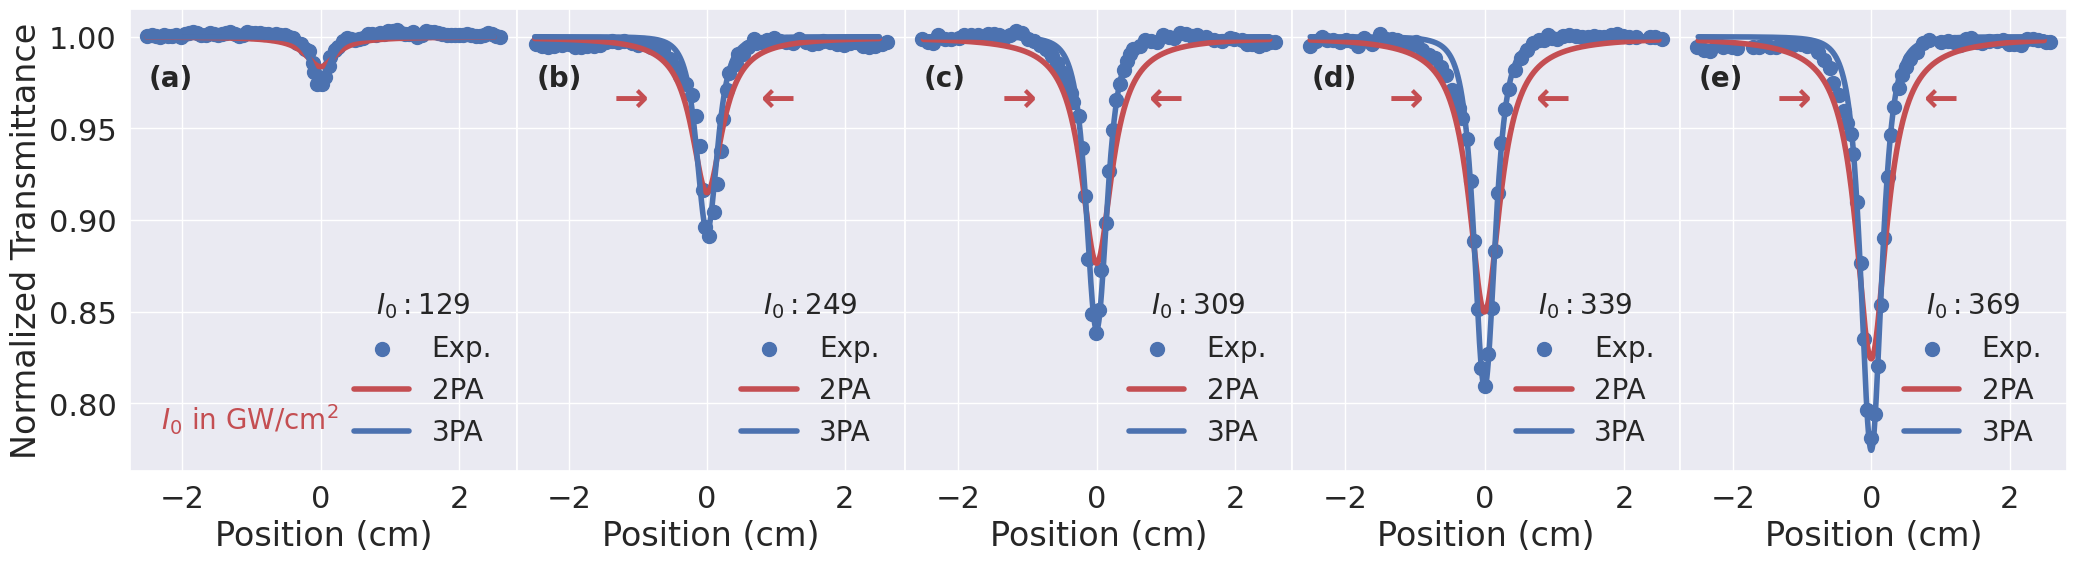
\includegraphics[width=\textwidth,keepaspectratio]{least1.png}
{\fontsize{35pt}{35pt}\selectfont  Figure 1: The Open Aperture Z-scan profiles with least square method of the material at different intensities.}
  \label{fig:least1}
\end{figure}      

\tcblower
\begin{tcolorbox}
[colback=white!60!lightgray,colframe=white!20!red]
\begin{figure}[H]    
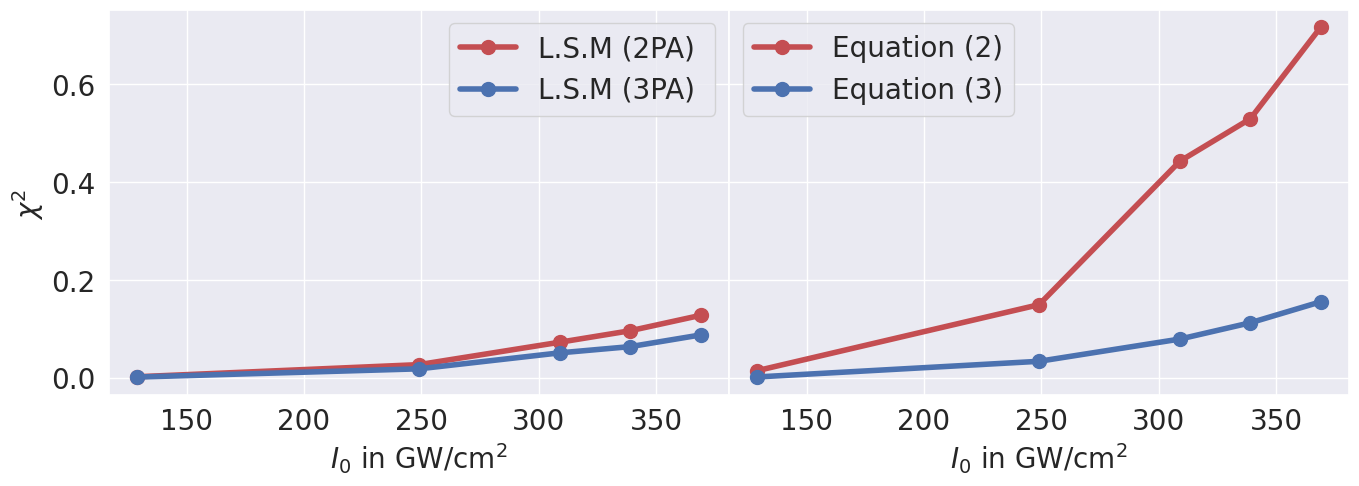
\includegraphics[width=\textwidth,keepaspectratio]{chsquare.png}
{\fontsize{35pt}{35pt}\selectfont  Figure 3: Comparison of $\chi^2$ under varying intensity for 2PA and 3PA.}
  \label{fig:absorption}
\end{figure}
\end{tcolorbox}
\end{Box1}
\begin{Box1}{}

\begin{figure}[H]    
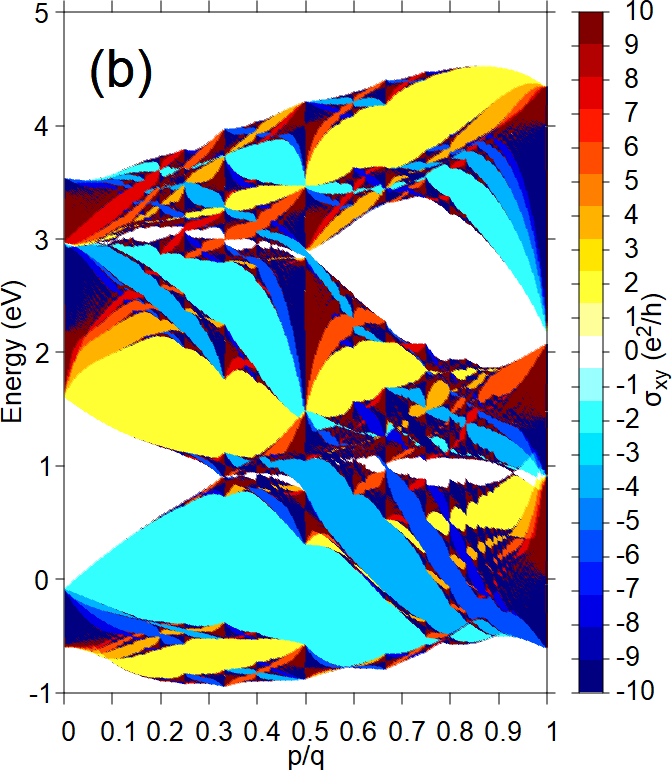
\includegraphics[width=0.25\linewidth,keepaspectratio]{images/3band_Chern_q_797_colorplane_f.png}
{\fontsize{35pt}{35pt}\selectfont  Figure 2: The Open Aperture Z-scan profiles with Eq$^n$-(2) and (3) of the material at different intensities.}
  \label{fig:absorption1}
\end{figure}      

\tcblower
\begin{tcolorbox}
[colback=white!60!lightgray,colframe=white!20!red]
\begin{table}[H]
\begin{longtable}{cccccccccc}
\caption{{\fontsize{35pt}{35pt}\selectfont Calculations of $\chi^2$, two ($\alpha_2$) and three ($\alpha_3$)-photon absorption coefficients.}}\\
\toprule
$I_0$ & \multicolumn{2}{c}{$\chi^2$ (2PA)} & \multicolumn{2}{c}{$\chi^2$ (3PA)} & \multicolumn{2}{c}{$\alpha_2$ (cm/W)} & \multicolumn{2}{c}{$\alpha_3$ (cm$^3$/W$^2$)}\\
\cmidrule(lr){2-3} \cmidrule(lr){4-5} \cmidrule(lr){6-7} \cmidrule(lr){8-9}
 (GW/cm$^{2}$) & L.S.M & Eq$^n$-(2) & L.S.M & Eq$^n$-(3) & L.S.M & Eq$^n$-(2) & L.S.M & Eq$^n$-(3) \\
 & & & & & ($\times 10^{-13}$) & ($\times 10^{-23}$) & ($\times 10^{-13}$) & ($\times 10^{-23}$)\\
\midrule
\endfirsthead

\multicolumn{10}{c}%
{{\tablename\ \thetable{} -- continued from previous page}} \\
\toprule
$I_0$ & \multicolumn{2}{c}{$\chi^2$ (2PA)} & \multicolumn{2}{c}{$\chi^2$ (3PA)} & \multicolumn{2}{c}{$\alpha_2$ (cm/W)} & \multicolumn{2}{c}{$\alpha_3$ (cm$^3$/W$^2$)}\\
\cmidrule(lr){2-3} \cmidrule(lr){4-5} \cmidrule(lr){6-7} \cmidrule(lr){8-9}
 & Fit & Eq$^n$-(2) & Fit & Eq$^n$-(3) & Fit & Eq$^n$-(2) & Fit & Eq$^n$-(3) \\
 & & & & & ($\times 10^{-13}$) & ($\times 10^{-23}$) & ($\times 10^{-13}$) & ($\times 10^{-23}$)\\
\midrule
\endhead

\midrule \multicolumn{10}{r}{{Continued on next page}} \\ \bottomrule
\endfoot

\bottomrule
\endlastfoot

129 & 0.0025 & 0.0149 & 0.0019 & 0.0021 & 1.08 & 0.56 & 1.35 & 8.10 \\
249 & 0.0273 & 0.1497 & 0.0187 & 0.0341 & 4.42 & 1.23 & 2.25 & 9.10 \\
309 & 0.0731 & 0.4429 & 0.0514 & 0.0795 & 4.71 & 1.47 & 1.98 & 8.78\\
339 & 0.0966 & 0.5297 & 0.0641 & 0.1128 & 5.58 & 1.59 & 2.12 & 8.61 \\
369 & 0.1281 & 0.7170 & 0.0880 & 0.1557 & 6.06 & 1.68 & 2.07 & 8.36 \\
\bottomrule

\end{longtable}
\end{table}
\end{tcolorbox}
\end{Box1}
\end{minipage}
}

\begin{multicols}{2}
    
% Conclusions
\coloredsection{accentorange!80!white}{Summary}{}
\coloredsubsection{accentorange!10!white}{
\begin{minipage}[t]{\linewidth}
We explored the Hofstadter butterfly spectrum in monolayer MoS\textsubscript{2} and related TMDs using a minimal three-band tight-binding model. Our results highlight the interplay between moiré superlattices and external magnetic fields, leading to quantum phenomena such as Landau levels and the integer quantum Hall effect (IQHE). This study demonstrates both the capabilities and limitations of tight-binding models in capturing topological effects in 2D materials.
\end{minipage}
}


\vspace{1cm}
% References
\coloredsection{lightgray!50!white}{References}{}
\coloredsubsection{lightgray!80!white}{
\begin{minipage}[t]{\linewidth}
    \renewcommand{\refname}{}
    \bibliographystyle{unsrt}
    \bibliography{refs}
\end{minipage}
}

\end{multicols}

% Acknowledgements
\coloredsection{vibrantblue!60!white}{Acknowledgements}{}

\vspace{0cm}
 
\coloredsubsection{vibrantblue!10!white}{
\Large We would like to acknowledge the professors, staff, and students of the Institute of Applied Mechanics and Informatics, VAST who provided support during this work.}


% \textit{Finally, I am very thankful to my wonderful friend \textbf{ Md. Fazle Rabbi Khan} who was beside me all the time, encouraging and inspiring me.}
     


\coloredsubsection{white!0}{
\begin{minipage}[t]{\linewidth}
    % \colorbox{highlightgreen!10!white}{%
        % \begin{minipage}{\textwidth}
            \begin{center}{\Large
               \textit{50th Vietnam Conference on Theoretical Physics (VCTP-50)}\\[1ex]
                 \textit{4-7 August, 2025 } | \textit{Dalat Palace Heritage.}}
            \end{center}
            \begin{center}
                \begin{tikzpicture}[remember picture,overlay]
                \node [anchor=south west] at ([xshift=0.5cm,yshift=1.25
                cm]current page.south west)
            {
\includegraphics[width=0.1\linewidth]          {images/VAST.png}}; 
                \end{tikzpicture}
                \end{center}
\end{minipage}
}



\end{document}
